\documentclass[10pt]{article}
\usepackage[polish]{babel}
\usepackage[utf8]{inputenc}
\usepackage[T1]{fontenc}
\usepackage{graphicx}
\usepackage[export]{adjustbox}
\graphicspath{ {./images/} }
\usepackage{amsmath}
\usepackage{amsfonts}
\usepackage{amssymb}
\usepackage[version=4]{mhchem}
\usepackage{stmaryrd}

\title{LIGA MATEMATYCZNA im. Zdzisława Matuskiego \\
 PÓŁFINAE \\
 29 lutego 2016 \\
 SZKOŁA PODSTAWOWA }

\author{}
\date{}


\begin{document}
\maketitle
\section*{ZADANIE 1.}
Kwadrat, którego długość boku jest równa 12, podzielono na mniejsze kwadraty (najmniejszy ma bok o długości 1) i prostokąty, które nie są kwadratami. Na rysunku podano długości boków niektórych figur. Które figury - kwadraty czy prostokąty - zajmują większą część dużego kwadratu?\\
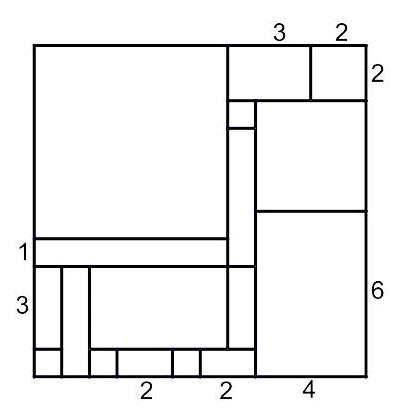
\includegraphics[max width=\textwidth, center]{2024_11_21_98eb331bc97ef7c88443g-1}

\section*{ZADANIE 2.}
Do liczby 36 dopisz po jednej cyfrze na końcu i na początku tak, aby otrzymana liczba czterocyfrowa była podzielna przez 36. Podaj wszystkie możliwości.

\section*{ZADANIE 3.}
Mama postawiła na stole tacę z cukierkami dla Ani, Bartka i Czarka. Ania wzięła trzecią część wszystkich cukierków, Bartek - trzecią część tego, co zostało na tacy. Na końcu Czarek wziął trzecią część reszty cukierków. Na tacy pozostały 24 cukierki. W jaki sposób mama powinna podzielić pozostałe cukierki, aby każde dziecko otrzymało jedną trzecią wszystkich cukierków?

\section*{ZADANIE 4.}
Wojtek wypisał 12 kolejnych liczb naturalnych w porządku rosnącym. Gdy dodał co drugą z nich, zaczynając od drugiej, otrzymał 3330. Jaką sumę uzyska, gdy doda co trzecią liczbę, zaczynając od trzeciej?

\section*{ZADANIE 5.}
Wykaż, że liczba \(\underbrace{3333 \ldots 35}_{2016 \text { cyfr } 3}\) jest podzielna przez 15.


\end{document}